% V3: control policy refiner with the solver as decoder (cost weights -> Riccati gains), under 5 pages.
% Based on the IEEE conference template (IEEEtran, conference mode), with small deviations
% (author block with advisors, tighter floats, smaller reference list).
\documentclass[conference]{IEEEtran}
\IEEEoverridecommandlockouts
\usepackage{cite}
\usepackage{amsmath,amssymb,amsfonts}
\usepackage{graphicx}
\usepackage{textcomp}
\usepackage{xcolor}
\usepackage{booktabs}
\usepackage{url}
\usepackage{tikz}
\usetikzlibrary{arrows.meta,positioning,calc,fit}

\newcommand{\R}{\mathbb{R}}
\newcommand{\T}{^{\top}}
\newcommand{\mpc}{\mathrm{MPC}}
\newcommand{\xb}{\bar{x}}
\newcommand{\ub}{\bar{u}}
\setlength{\textfloatsep}{8pt plus 2pt minus 2pt}
\setlength{\dbltextfloatsep}{8pt plus 2pt minus 2pt}
\setlength{\abovecaptionskip}{3pt}

\begin{document}

\title{Control Policy Refiner in Legged Robotics:\\ Preliminary Results}

\author{\IEEEauthorblockN{Norawit Nangsue\textsuperscript{1,2}}
\IEEEauthorblockA{Advisors: Fumio Kanehiro\textsuperscript{1,2} and Mehdi Benallegue\textsuperscript{2}}
\IEEEauthorblockA{\textsuperscript{1}University of Tsukuba, Ibaraki, Japan}
\textsuperscript{2}CNRS-AIST JRL (Joint Robotics Laboratory), IRL,\\
National Institute of Advanced Industrial Science and Technology (AIST), Japan\\
}

\maketitle

\begin{abstract}
A model predictive controller (MPC) based on differential dynamic programming provides a feedback policy, made of a state set-point and a gain matrix, that drives a humanoid robot between two solves.
This policy is optimal for the model, not for the robot.
We propose a \emph{control policy refiner} that makes the robot system more robust to uncertainty by using residual reinforcement learning (ResRL) policy that outputs a few cost-weight scales and a set-point shift such that it improves the overall behavior.
The solver is used as a decoder: one Riccati backward pass along the current trajectory turns the modified weights into a full gain matrix.
Every gain the refiner can produce is therefore the optimal feedback of a valid local problem, which keeps exploration safe and the action space small (about 17 numbers instead of 432).
As the base controller, we implemented an IS-MPC gait generator with a reformulated footstep timing and position pre-optimization and a whole-body MPC of the HRP-5P legs.
In MuJoCo it walks at up to 0.3\,m/s with a mean whole-body solve time of 6.7\,ms and recovers from 26 of 36 pushes.
The refiner itself has not been trained yet.
\end{abstract}

\begin{IEEEkeywords}
humanoid robots, model predictive control, residual reinforcement learning, feedback gains modification, setpoint modification 
\end{IEEEkeywords}

\section{Introduction}

Model-based controllers make a humanoid walk by planning with a reduced model such as the linear inverted pendulum (LIPM) \cite{kajita2001lipm} and tracking the plan with a whole-body controller, increasingly a whole-body MPC \cite{mastalli2020crocoddyl,dantec2022wbmpc}.
Learning-based controllers train a neural network policy in simulation with RL \cite{radosavovic2024humanoid}.
An MPC handles constraints explicitly and can be re-targeted without retraining, but it is optimal only for its model, which leaves out joint flexibility, contact compliance and actuator dynamics.
An RL policy absorbs such effects from experience, but it is a black box.

The usual way to combine them is residual RL \cite{johannink2019residual}: the model-based controller is kept and a learned correction is added to its output, as a joint torque or position target \cite{jenelten2024dtc,jeon2025residualmpc}.
Such a correction is unstructured, with one free number per joint at every control step and nothing tying it to the model that produced the base action.

A whole-body MPC solved by differential dynamic programming (DDP) \cite{mayne1966ddp} offers a more structured place for learning.
The solver returns Riccati gains with the torque trajectory, and together they form a feedback policy, with a set-point and a reactiveness, that drives the robot between two solves \cite{grandia2019feedback,dantec2022firstorder}.
In existing work these gains are applied as computed.
Our goal is to make this feedback policy robust to uncertainty by letting a learned policy, the \emph{refiner}, adjust it online.

Learning the gains directly is not practical: for the leg model they have 432 entries per node, and an arbitrary change can destabilize the robot.
We instead let the refiner act on the \emph{cost} from which the gains are computed and use the solver as a decoder.
Policies that set the parameters of an MPC exist: for the decision variables of a quadrotor MPC \cite{song2022policysearch}, for a learned cost in a differentiable MPC \cite{romero2024acmpc}, and in theory for an MPC used as a parametrized policy \cite{gros2020nmpcrl}.
They re-solve the MPC with the new parameters, which changes the planned motion.
Our refiner keeps the plan and changes only the reaction: the weights are decoded by one backward pass, between two solves, into new gains, in the spirit of variable impedance learning \cite{buchli2011variable}.

This report presents (i) the refiner and its decoder (Section~\ref{sec:method}), (ii) the base controller it refines (Section~\ref{sec:base}), and (iii) simulation results of the base controller that show what has to be corrected (Section~\ref{sec:results}).

\section{Base Controller}
\label{sec:base}

\begin{figure*}[t]
\centering
\resizebox{\textwidth}{!}{%
\begin{tikzpicture}[font=\footnotesize, >={Stealth[length=1.6mm]},
  blk/.style={draw, rounded corners=1.5pt, minimum height=10mm, align=center, inner sep=2.5pt, fill=black!4},
  grp/.style={draw, dashed, rounded corners=3pt, inner sep=5pt, inner ysep=7pt},
  lab/.style={font=\scriptsize, align=center}]
\node[lab] (cmd) {velocity\\command};
\node[blk, right=4mm of cmd] (ftpp) {Candidate steps +\\pre-optimization\\{\scriptsize NLP (IPOPT)}};
\node[blk, right=3.5mm of ftpp] (ismpc) {IS-MPC\\{\scriptsize QP (OSQP)}};
\node[blk, right=3.5mm of ismpc] (roll) {LIPM rollout,\\swing traj.};
\node[blk, right=12mm of roll] (ocp) {OCP of the legs\\{\scriptsize 18 DoF, $25\times20$\,ms}};
\node[blk, right=3.5mm of ocp] (ddp) {FDDP\\solver};
\node[blk, right=9mm of ddp] (ric) {Feedback policy\\$\tau=\ub+K(\xb\ominus x)$};
\node[inner sep=0pt, right=5mm of ric] (rob) {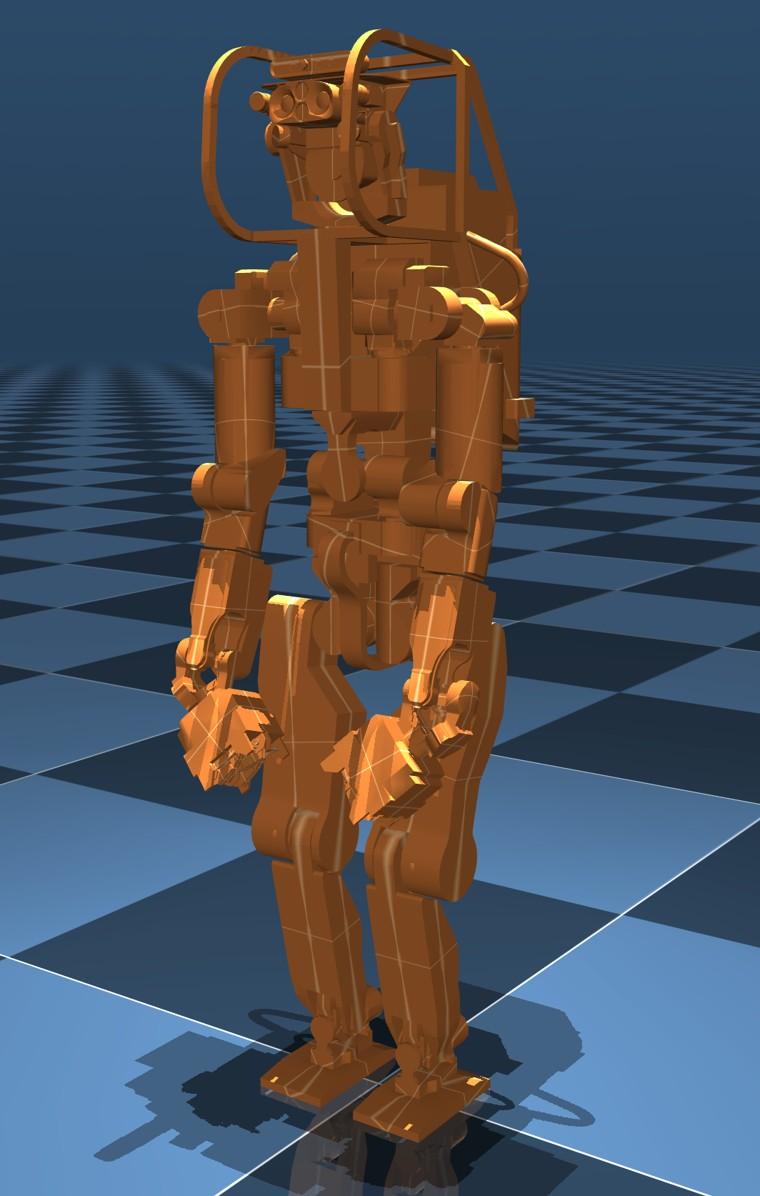
\includegraphics[height=27mm]{figures/hrp5p.jpg}};
\node[grp, fit=(ftpp)(ismpc)(roll)] (gg) {};
\node[grp, fit=(ocp)(ddp)] (wb) {};
\node[lab, above=0.2mm of gg.north] {\textbf{Gait generator} (LIPM), 20\,Hz};
\node[lab, above=0.2mm of wb.north] {\textbf{Whole-body MPC} (Crocoddyl), 10\,Hz};
\node[lab, above=0.2mm of ric.north] {1\,kHz};
\node[lab, below=0.2mm of rob.south] {HRP-5P in MuJoCo};
\draw[->] (cmd) -- (ftpp);
\draw[->] (ftpp) -- (ismpc);
\draw[->] (ismpc) -- (roll);
\draw[->] (roll) -- node[lab, above] {refs.} (ocp);
\draw[->] (ocp) -- (ddp);
\draw[->] (ddp) -- node[lab, above] {$\xb,\ub,K$} (ric);
\draw[->] (ric) -- node[lab, above] {$\tau$} (rob);
\coordinate (fb) at ($(ric.south)+(0,-9mm)$);
\draw[->] (rob.west |- fb) -- (fb) -- (ric.south);
\draw[->] (fb) -| node[lab, pos=0.2, below] {state $x$} (ocp.south);
\draw[->] (fb -| ocp.south) -| node[lab, pos=0.2, below] {measured DCM} (ismpc.south);
\end{tikzpicture}}
\caption{Base controller: an IS-MPC gait generator sends CoM, foot and contact references to a whole-body MPC built on Crocoddyl, whose feedback policy is evaluated at 1\,kHz on the HRP-5P model in MuJoCo (image rendered from the simulation).}
\label{fig:base}
\end{figure*}

Fig.~\ref{fig:base} shows the base controller.

\subsection{Gait generator}
With CoM $c$, ZMP $p$ and $\eta=\sqrt{g/z_c}$, the divergent component of motion (DCM) $\xi=c+\dot c/\eta$ obeys $\dot\xi=\eta(\xi-p)$.
It stays bounded if and only if \cite{lanari2014boundedness}
\begin{equation}
\xi(t_0)=\eta\int_{0}^{\infty}e^{-\eta\tau}\,p(t_0+\tau)\,d\tau .
\label{eq:stab}
\end{equation}
IS-MPC \cite{scianca2020ismpc} enforces \eqref{eq:stab} as a constraint of a QP on the ZMP velocity and the footsteps.
After a push, \eqref{eq:stab} may be infeasible with the nominal step times, so the footstep positions $p_f^k$ and times $t_k$ are first adjusted by a pre-optimization \cite{dallard2025adios}, written with $\mu_k=e^{-\eta t_k}$.
This problem is badly scaled, since $\mu_k$ reaches $10^{-7}$ at the end of the preview, and the reference implementation \cite{ismpcwalking} solves it by block coordinate descent, dropping the divisor of the displacement term.
We replace $\mu_k$ by the ratio $\nu_k=\mu_k/\hat\mu_k$ to its nominal value, which makes all variables of order one, keep the original cost
\begin{multline}
J=\sum_k(\nu_k-1)^2+w_s\|s\|^2\\
+K_s\sum_{i\ge1}\big\|p_f^i-\hat p_f^i\big\|^2\,
\frac{(\nu_i\hat\mu_i-\nu_{i-1}\hat\mu_{i-1})^2}{(\hat\mu_i-\hat\mu_{i-1})^2},
\label{eq:cost}
\end{multline}
where $s$ is the slack of the DCM condition, and solve positions and times jointly as one nonlinear program with CasADi \cite{andersson2019casadi} and IPOPT \cite{wachter2006ipopt}.
The IS-MPC QP then uses the result as candidates and is solved with OSQP \cite{stellato2020osqp}.
The generator replans at every touchdown and re-solves the QP every 50\,ms; it includes capture steps and a DCM feedback law for standing.

\subsection{Whole-body MPC and its feedback policy}
The optimal control problem (OCP) uses the floating base and the twelve leg joints of HRP-5P \cite{kaneko2019hrp5p} ($n_v=18$), with rigid 6D contacts that follow the gait generator's schedule.
Its running cost is a weighted sum of residuals,
\begin{equation}
\ell(x,u)=\tfrac12\sum_{c}w_c\,\|r_c(x,u)\|^2_{W_c},
\label{eq:costwb}
\end{equation}
with terms for the CoM, the feet, the posture (base orientation, joint positions, velocities) and the torques.
It is solved with the FDDP solver of Crocoddyl \cite{mastalli2020crocoddyl} every 100\,ms, and each solve returns the trajectories $\xb_i,\ub_i$ and the Riccati gains $K_i$.
Between solves, the torque is
\begin{equation}
\tau^{\mpc}=\ub_i+K_i\,(\xb_i\ominus x),\qquad K_i\in\R^{12\times36},
\label{eq:riccati}
\end{equation}
evaluated at 1\,kHz with the measured state $x$.
The 36 columns of $K_i$ are the errors of the base pose (6), the joint positions (12), the base velocity (6) and the joint velocities (12).

\section{Control Policy Refiner}
\label{sec:method}

\begin{figure}[t]
\centering
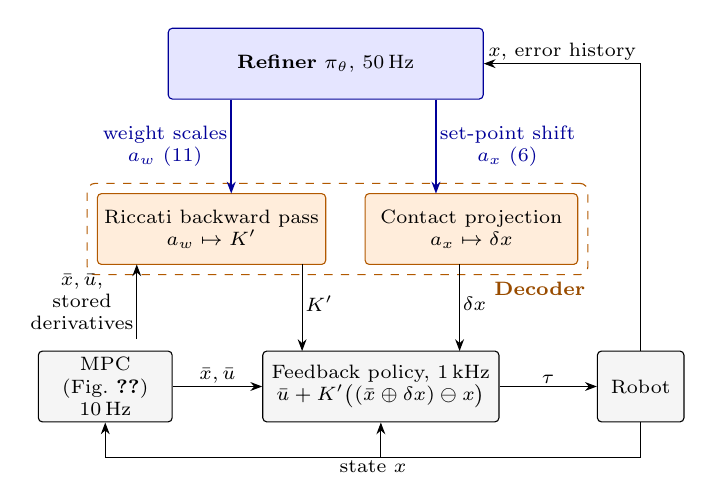
\begin{tikzpicture}[x=1mm, y=1mm, font=\scriptsize, >={Stealth[length=1.5mm]},
  blk/.style={draw, rounded corners=1.5pt, minimum height=9mm, align=center, inner sep=2pt, fill=black!4},
  res/.style={draw, rounded corners=1.5pt, minimum height=9mm, align=center, inner sep=2pt, fill=blue!10, draw=blue!60!black},
  dec/.style={draw, rounded corners=1.5pt, minimum height=9mm, align=center, inner sep=2pt, fill=orange!14, draw=orange!70!black},
  lab/.style={font=\scriptsize, align=center, inner sep=1pt}]
\node[blk, minimum width=17mm] (mpc) at (0,0) {MPC\\(Fig.~\ref{fig:base})\\10\,Hz};
\node[blk, minimum width=30mm] (fb) at (35,0) {Feedback policy, 1\,kHz\\$\ub+K'\big((\xb\oplus\delta x)\ominus x\big)$};
\node[blk, minimum width=11mm] (rob) at (68,0) {Robot};
\node[dec, minimum width=29mm] (bp) at (13.5,20) {Riccati backward pass\\$a_w\mapsto K'$};
\node[dec, minimum width=27mm] (pr) at (46.5,20) {Contact projection\\$a_x\mapsto\delta x$};
\node[draw=orange!70!black, dashed, rounded corners=3pt, inner sep=3.5pt, fit=(bp)(pr)] (decgrp) {};
\node[lab, text=orange!60!black, anchor=north east] at ($(decgrp.south east)+(0,-0.5)$) {\textbf{Decoder}};
\node[res, minimum width=40mm] (pol) at (28,41) {\textbf{Refiner} $\pi_\theta$, 50\,Hz};
\draw[->, blue!60!black, thick] (pol.south -| 16,0) -- node[lab, left, text=blue!60!black] {weight scales\\$a_w$ (11)} (16,24.5);
\draw[->, blue!60!black, thick] (pol.south -| 42,0) -- node[lab, right, text=blue!60!black] {set-point shift\\$a_x$ (6)} (42,24.5);
\draw[->] (4,6) -- node[lab, left] {$\xb,\ub$,\\stored\\derivatives} (4,15.5);
\draw[->] (25,15.5) -- node[lab, right, pos=0.45] {$K'$} (25,4.5);
\draw[->] (45,15.5) -- node[lab, right, pos=0.45] {$\delta x$} (45,4.5);
\draw[->] (mpc) -- node[lab, above] {$\xb,\ub$} (fb);
\draw[->] (fb) -- node[lab, above] {$\tau$} (rob);
\draw[->] (rob.south) -- (68,-9) -| node[lab, pos=0.25, below] {state $x$} (mpc.south);
\draw[->] (68,-9) -| (fb.south);
\draw[->] (rob.north) -- (68,41) -- node[lab, above] {$x$, error history} (pol.east);
\end{tikzpicture}
\caption{The refiner stack. The MPC of Fig.~\ref{fig:base} is treated as one block. The refiner outputs 17 numbers; the decoder turns them into a full gain matrix $K'$, by one backward pass of the solver, and into a contact-consistent set-point shift $\delta x$. The refiner never outputs a torque or a gain directly.}
\label{fig:stack}
\end{figure}

\subsection{Overview}
In \eqref{eq:riccati}, the set-point $\xb$ says where the robot should be, and the gain $K$ says how strongly, and through which joints, it reacts when it is not there.
Each MPC solution is executed for 100 control steps, so this law alone determines the behaviour in that interval, and it is the law that meets the uncertainty: a push, a wrong mass, a softer floor.
The refiner (Fig.~\ref{fig:stack}) adjusts both parts,
\begin{equation}
\tau=\ub+K'\,\big((\xb\oplus\delta x)\ominus x\big),
\label{eq:refined}
\end{equation}
at the node rate of 50\,Hz.
It outputs a latent $a=(a_w,a_x)$, and a fixed decoder maps $a_w$ to the gain $K'$ and $a_x$ to the shift $\delta x$.
The decoder is not learned: RL explores in the latent, and $a=0$ gives exactly the base controller.

\subsection{Solver as decoder for the gains}
The Riccati gains are a function of the cost \eqref{eq:costwb}.
The refiner scales its weights,
\begin{equation}
w_c\leftarrow w_c\,e^{a_{w,c}},
\label{eq:scale}
\end{equation}
and the decoder runs the backward pass of the solver once more along the current trajectory.
With the Gauss--Newton approximation used by the solver, the cost Hessian is linear in the weights, $\ell_{xx}=\sum_c w_c\,J_c\T W_cJ_c$ (and similarly for $\ell_{ux},\ell_{uu}$), so it is a weighted sum of blocks already computed by the last solve.
The dynamics Jacobians $f_x,f_u$ are also stored.
The recursion, from the last node to the first, is
\begin{align}
Q_{uu}&=\ell_{uu}+f_u\T V'_{xx}f_u, &Q_{ux}&=\ell_{ux}+f_u\T V'_{xx}f_x,\nonumber\\
Q_{xx}&=\ell_{xx}+f_x\T V'_{xx}f_x, &K'&=Q_{uu}^{-1}Q_{ux},\nonumber\\
V_{xx}&=Q_{xx}-Q_{ux}\T K', &&
\label{eq:backward}
\end{align}
where $V'_{xx}$ is the value Hessian of the next node.
Only the gains are used.
The feedforward torque and the set-point of the last solve are kept, so the decoded gains change the reaction and not the planned motion.

The weight scales are of two kinds (Table~\ref{tab:latent}).
\emph{Tracking weights} set what the feedback protects: the CoM, the base orientation, the joint posture, the velocities (damping) and the feet.
\emph{Torque weights}, one per joint group, set how much each joint is trusted to react: raising the torque weight of the stance ankle softens it, and the rest of the gain adapts so that the hip and the knee take over.
Raising all torque weights lowers the bandwidth of the feedback, which is the classical remedy against unmodelled dynamics.

\begin{table}[t]
\caption{Latent of the refiner}
\label{tab:latent}
\centering
\setlength{\tabcolsep}{3pt}
\resizebox{\columnwidth}{!}{%
\begin{tabular}{@{}llc@{}}
\toprule
Part & Content & Size\\
\midrule
$a_w$, tracking & CoM, base orientation, posture, velocities, feet & 5\\
$a_w$, torque & hip, knee, ankle of the stance and the swing leg & 6\\
$a_x$ & base pose shift; leg joints by contact projection & 6\\
\midrule
\multicolumn{2}{@{}l}{Decoded: $K'\in\R^{12\times36}$ per node, and $\delta x\in\R^{36}$} & 17\\
\bottomrule
\end{tabular}}
\end{table}

\subsection{Set-point shift}
The shift is output directly, restricted to configurations that keep the stance feet in place:
\begin{equation}
\delta x=\begin{bmatrix}P_c\,S\,a_x\\ 0\end{bmatrix},\qquad P_c=I-J_c^{+}J_c ,
\label{eq:setpoint}
\end{equation}
where $S$ selects the base pose and $J_c$ is the Jacobian of the feet in contact, so the refiner outputs a change of the base pose and the projection completes the leg joints.
The resulting torque $K'\delta x$ lies in the range of the gain.
Since the Riccati policy is the first-order expansion of the MPC solution with respect to the state \cite{dantec2022firstorder}, it is the torque the MPC itself would command if the robot were displaced by $-\delta x$: the refiner acts as a learned bias on the state seen by the controller.
It handles what a gain cannot, namely steady errors such as a CoM offset.

\subsection{Properties and limits}
\emph{Safe by construction.} With positive weights, $Q_{uu}$ is positive definite and $K'$ is the optimal feedback of a valid local linear-quadratic problem.
The refiner can choose a poor cost, but it cannot produce a gain with flipped signs or with a broken coupling between joints, and $K'$ is consistent with the contacts because it is computed through the same contact-constrained dynamics, a condition for using such gains on hardware \cite{grandia2019feedback}.

\emph{Small and meaningful.} The latent has 17 numbers, each with a physical meaning that can be bounded and inspected, and the decoded gain depends smoothly on it.

\emph{Cheap.} The decoder is a weighted sum and one recursion over 25 nodes, without new derivatives; a complete solver iteration takes about 0.8\,ms in our implementation, which bounds its cost.

\emph{Limits.} The decoder only reaches gains that are optimal for some cost on the model's dynamics.
If the dynamics themselves are wrong, the best gain may lie outside this family, and the refiner can then only detune.
The gains do not respond evenly to the weights, so the bound of each scale must be calibrated, and the scales are rate-limited because a fast-varying gain can destabilize a loop even when every frozen value is stabilizing.
The refiner cannot change the footsteps or the contact schedule: disturbances that need a different step remain the task of the gait generator.

\subsection{Learning for robustness}
The refiner observes the state, a short history of tracking errors and torques, the contact flags and step phase, the velocity command and its previous output.
The history lets it recognize the situation, for example a heavier robot or a softer floor, and choose weights accordingly, instead of learning one compromise setting.
It is trained with PPO \cite{schulman2017ppo} in simulation under the uncertainties it should withstand: pushes, mass and CoM offsets, friction, contact stiffness and actuation delay.
The reward combines velocity tracking and staying upright with penalties on the size and rate of the latent, on joint torques, on a centre of pressure (CoP) near the sole edge and on a tilted stance foot.
The MPC and the decoder are part of the environment, so no derivative of the solver is needed.

\section{Preliminary Results: Base Controller}
\label{sec:results}

The refiner has not been trained; this section reports the base controller alone.
The HRP-5P model (104\,kg) is simulated in MuJoCo \cite{todorov2012mujoco} with a 1\,ms step and torque control, with $z_c=1.014$\,m and steps of at most 0.8\,s.
Runs are headless on one thread of a laptop (Apple M5).
A fall is a base height below 0.5\,m.
A push is an instantaneous change of the base velocity $\Delta v=\eta d$, which shifts the DCM by $d$ ($d=0.08$\,m is 0.25\,m/s, about 26\,N\,s).

\begin{table}[t]
\caption{Walking in simulation (base controller, no falls)}
\label{tab:walk}
\centering
\setlength{\tabcolsep}{3pt}
\resizebox{\columnwidth}{!}{%
\begin{tabular}{@{}lcccccc@{}}
\toprule
Command & Dist. & Steps & \multicolumn{2}{c}{Error (max) [mm]} & CoP & Solve [ms]\\
 & [m] & & foot & DCM & ratio$^{\mathrm a}$ & mean / max\\
\midrule
0.2\,m/s & 0.93 & 8 & 18 & 28 & 1.45 & 6.4 / 14.2\\
0.3\,m/s, 0.2\,rad/s & 1.46 & 9 & 31 & 40 & 1.81 & 6.9 / 10.0\\
$-0.15$\,m/s & 0.74 & 8 & 10 & 30 & 1.47 & 6.1 / 8.7\\
0.3\,m/s (8\,s) & 2.43 & 13 & 30 & 36 & 1.59 & 7.1 / 11.6\\
\bottomrule
\multicolumn{7}{@{}l}{$^{\mathrm a}$Largest measured CoP offset of a stance foot divided by the half-size}\\
\multicolumn{7}{@{}l}{\phantom{$^{\mathrm a}$}of the largest centred box inside the sole; above 1 is near the sole edge.}
\end{tabular}}
\end{table}

\begin{table}[t]
\caption{Pushes survived, by DCM shift $d$ (four directions each)}
\label{tab:push}
\centering
\setlength{\tabcolsep}{4pt}
\begin{tabular}{@{}lcccccc@{}}
\toprule
\multicolumn{7}{@{}l}{\emph{Standing}}\\
$d$ [m] & 0.04 & 0.06 & 0.08 & 0.10 & 0.12 & Total\\
\midrule
Push detection on (default) & 4/4 & 4/4 & 4/4 & 1/4$^{\mathrm a}$ & 0/4 & 13/20\\
Push detection off & 4/4 & 4/4 & 2/4 & 1/4 & 0/4 & 11/20\\
\midrule
\multicolumn{7}{@{}l}{\emph{Walking at 0.2\,m/s} (two push instants)}\\
$d$ [m] & \multicolumn{2}{c}{0.05} & \multicolumn{2}{c}{0.08} & & Total\\
\midrule
Default & \multicolumn{2}{c}{7/8} & \multicolumn{2}{c}{6/8} & & 13/16\\
\bottomrule
\multicolumn{7}{@{}l}{$^{\mathrm a}$Two further cases stay up on a tilted foot and are not counted.}
\end{tabular}
\end{table}

\emph{Walking.} The robot does not fall in any of the four commands of Table~\ref{tab:walk} (5\,s each, 8\,s in the last row).
The measured DCM follows the planned one with an RMS error of 12 to 16\,mm.
The whole-body solve takes 6.7\,ms on average (8.2 iterations) and at most 14.2\,ms of the 100\,ms period; a touchdown replan of the gait generator takes 7.2\,ms on average.

\emph{Pushes.} The robot recovers from 26 of the 36 pushes of Table~\ref{tab:push}.
The failures are directional: while walking, the three falls are pushes toward the robot's right; while standing at 0.10\,m, they are the backward and the two lateral pushes.

\emph{What the refiner has to correct.}
(1)~\emph{Contact moments.} The CoP ratio exceeds 1 in every run, and after strong lateral pushes a stance foot rolls onto its edge.
The OCP has no limit on the CoP, so its plan and its feedback ask for ankle moments the sole cannot transmit; a wrench-cone penalty in the cost made walking fail.
A higher torque weight on the stance ankle reduces the moment the feedback asks for, and a base shift toward the stance foot reduces the moment the plan needs.
(2)~\emph{Tracking lag.} The robot lags the LIPM reference by 3 to 4\,cm of DCM in single support, systematically and depending on the step phase, which a set-point shift can lead.
(3)~\emph{Reaction to pushes.} The reaction that fails is the one computed for the nominal cost on the unperturbed plan; which weights give a reaction that recovers is what the refiner is meant to learn.
Lateral step limits are narrow ($\pm3.5$\,cm), so part of the lateral failures need a different step and are outside its reach.

\section{Plan and Conclusion}
\label{sec:plan}

We proposed to refine the feedback policy of a whole-body MPC with a learned policy that acts on the cost weights and on the set-point, using one backward pass of the solver as a decoder.
The refiner stays within gains that are optimal for the model, which makes learning safe and low-dimensional, and aims at robustness to uncertainty and not at a new motion.
The base controller is implemented and walks in simulation, and its weaknesses map to the two parts of the latent.

The next steps are: to implement the decoder in Crocoddyl and calibrate the bounds of the latent; to train the refiner under the randomized uncertainties above; and to compare it, on the protocols of Tables~\ref{tab:walk} and~\ref{tab:push} with randomized mass, friction and delay, against the base controller, a direct scaling of the gains, and an unstructured torque residual.
If the refiner fails specifically on delay or contact compliance, that will indicate that the model's dynamics, and not its cost, are the bottleneck.
With the measured solve times, $10^8$ refiner steps at 50\,Hz cost in the order of 100 core-hours of MPC and decoding, which is feasible on CPUs.
After simulation, the controller needs a state estimator and a port to mc\_rtc for experiments on HRP-5P.

% slightly smaller, tighter reference list (deviation from the IEEE template to stay within 4 pages)
\begingroup
\renewcommand{\footnotesize}{\fontsize{7.3}{8.3}\selectfont}
\setlength{\itemsep}{0pt}
\bibliographystyle{IEEEtran}
\bibliography{refs}
\endgroup

\end{document}
